\graphicspath{{members/ssr/figures/}}

\subsubsection{Camera Setup}
\input{members/ssr/authors}

The input data for Pipeline A is acquired through a digital photo camera which is mounted above the
plants and can move along each lane and take an image from every single plant.
Each captured image contains a square of a ground unit which shows only one plant from above
showing it's canopy, as shown in figure \ref{fig:pipeline:a:camera:setup}

\begin{figure}[H]
    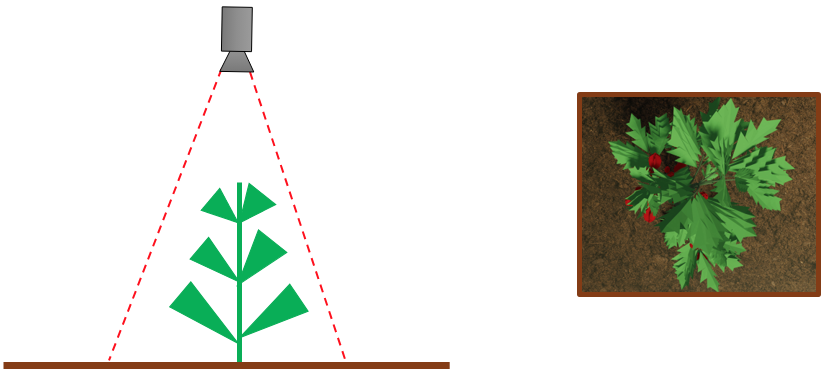
\includegraphics[width=\textwidth,height=\textheight,keepaspectratio]{modelling/camera-setup.png}
    \caption{Camera setup for input data for Pipeline A. Right: Canopy image taken by the camera}
    \label{fig:pipeline:a:camera:setup}
\end{figure}

This basic metric is fed into the pipeline for further processing.
Its purpose is to measure the canopy size which is done by segmentation, as presented in the next chapter.